\documentclass[11pt]{beamer}
%
% Choose how your presentation looks.
%
% For more themes, color themes and font themes, see:
% http://deic.uab.es/~iblanes/beamer_gallery/index_by_theme.html
%
	\definecolor{bostonuniversityred}{rgb}{0.8, 0.0, 0.0}
\mode<presentation>
{
  \usetheme{Madrid}      % or try Darmstadt, Madrid, Warsaw, ...
  \usecolortheme{beaver} % or try albatross, beaver, crane, ...
  \usefonttheme{default}  % or try serif, structurebold, ...
  \setbeamertemplate{navigation symbols}{}
  \setbeamertemplate{caption}[numbered]
} 
%\usepackage{pifont}
\usepackage{listings}
\usepackage{euler}
\usepackage{tikz}
\usepackage{bm}
\usetikzlibrary{bayesnet}
\usetikzlibrary{arrows}
\usepackage{bbm}
\usetheme[secheader]{Boadilla}
\usecolortheme[named=bostonuniversityred]{structure}
\usepackage[bookmarks]{hyperref}
\usepackage[backend=bibtex]{biblatex}
\usepackage[a-3u]{pdfx} 
\setbeamercolor{title}{parent=author in head/foot}
\usepackage{braket}
\usepackage{amsmath,amsfonts,amsthm,bm}
\addbibresource{bibliography.bib}
\newtheorem*{remark}{Remark}
\usepackage[italian]{babel}
\usepackage[utf8x]{inputenc}
\usebackgroundtemplate{\includegraphics[width=\paperwidth]{Pic/Cover_image.png}}
\title[Review]{Time series}
\author{Marzio De Corato}
\date{\today}

\begin{document}

\begin{frame}
\vspace{+6.9 cm}  \titlepage
\end{frame}

\usebackgroundtemplate{ } 

\section{Preliminary definitions}


\begin{frame}
\begin{center}
\Huge
Preliminary definitions
\end{center}
\end{frame}

\begin{frame}{Time series definition \cite{brockwell2002introduction}}
\begin{alertblock}{Informal definition}
A time-series is a set of observation $x_{t}$ each one being recorder at a specific time t. 
\end{alertblock}
\begin{alertblock}{Formal definition }
A time series model for the observed data ${x}_{t}$ is a specification of the joint distribution (or possible only the means covariance) of a sequence of random variable ${X}_{t}$ of which ${x}_{t}$ is postulated to be a realization
\end{alertblock}
\begin{exampleblock}{A binary process}
Consider the sequence of iid random variables, with $P[X_{t}=1]=p$ and $P[X_{t}=-1]=1-p$
\end{exampleblock}
\begin{exampleblock}{Random walk}
The random walk is obtained by cumulatively summing iid random variables. Thus a random walk with zero mean is obtained by defining $S_{0}=0$ and $S_{t}=X_{1}+X_{2}+...+X_{t}$ for $t=1,2,..$ where ${X_{t}}$ a iid noise. 
\end{exampleblock}
\end{frame}


\begin{frame}{Stationarity, autocovariance and autocorrelation\cite{brockwell2002introduction}}
\begin{alertblock}{Mean Function}
Let ${X_{t}}$ be a time series with $E({x}_{t}^{2}< \infty$  The mean function of ${X_{t}}$ is $\mu_{X}(t)=E(X_{t})$. The covariance function of ${X_{t}}$ is $\gamma_{X}(r,s)=Cov(X_{r},X_{S})=E[(X_{r}-\mu_{X}(r))(X_{s}-\mu_{X}(s))]\quad\forall r,s$ 
\end{alertblock}
\begin{alertblock}{Weakly stationary TS}
${X_{t}}$ is weakly stationary if i) $\mu_{X}(t)$ is independent from time t and ii) $\gamma_{X}(t+h)$ is indipendent of t $\forall h$
\end{alertblock}
\begin{alertblock}{Autocovariance function}
At lag h the auto-covariance function is defined as $\gamma_{X}(h)=Cov(X_{t+h},X_{t})$ 
\end{alertblock}
\begin{alertblock}{Autocorrelation function}
At lag h the autocorrelation function is defined as $\rho(h)_{X}=\dfrac{\gamma_{X}(h)}{\gamma_{X}(0)}=Cor({X}_{t+h},{X}_{t})$ 
\end{alertblock}
\end{frame}

\begin{frame}{Stationarity, autocovariance and autocorrelation \cite{brockwell2002introduction}}
    \begin{center}
     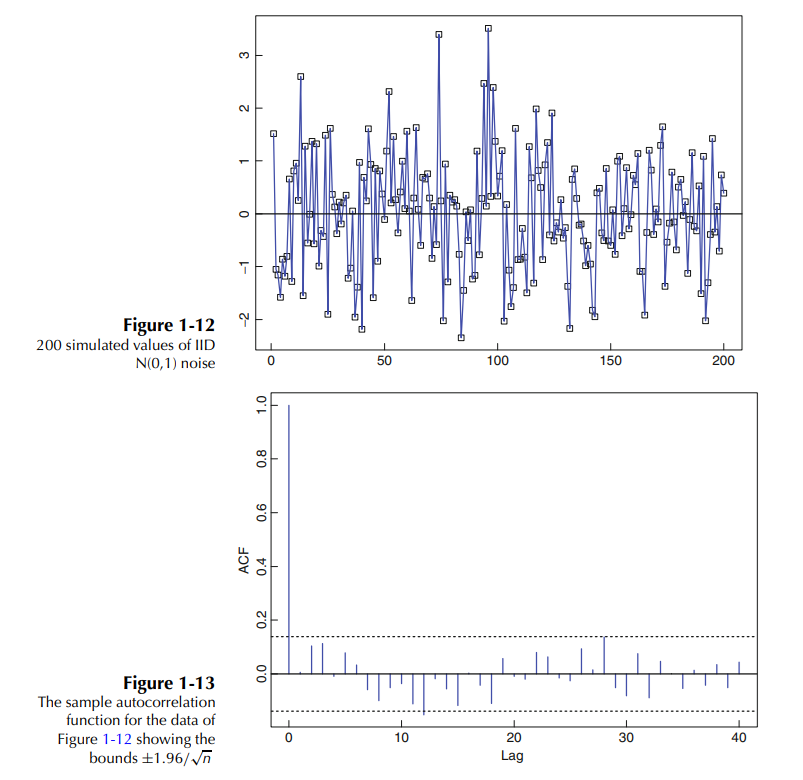
\includegraphics[width=0.6\textwidth]{Pic/ACF.png}
    \end{center}
\end{frame}

\begin{frame}{Stationarity, autocovariance and autocorrelation \cite{hao2024improving}}
    \begin{center}
     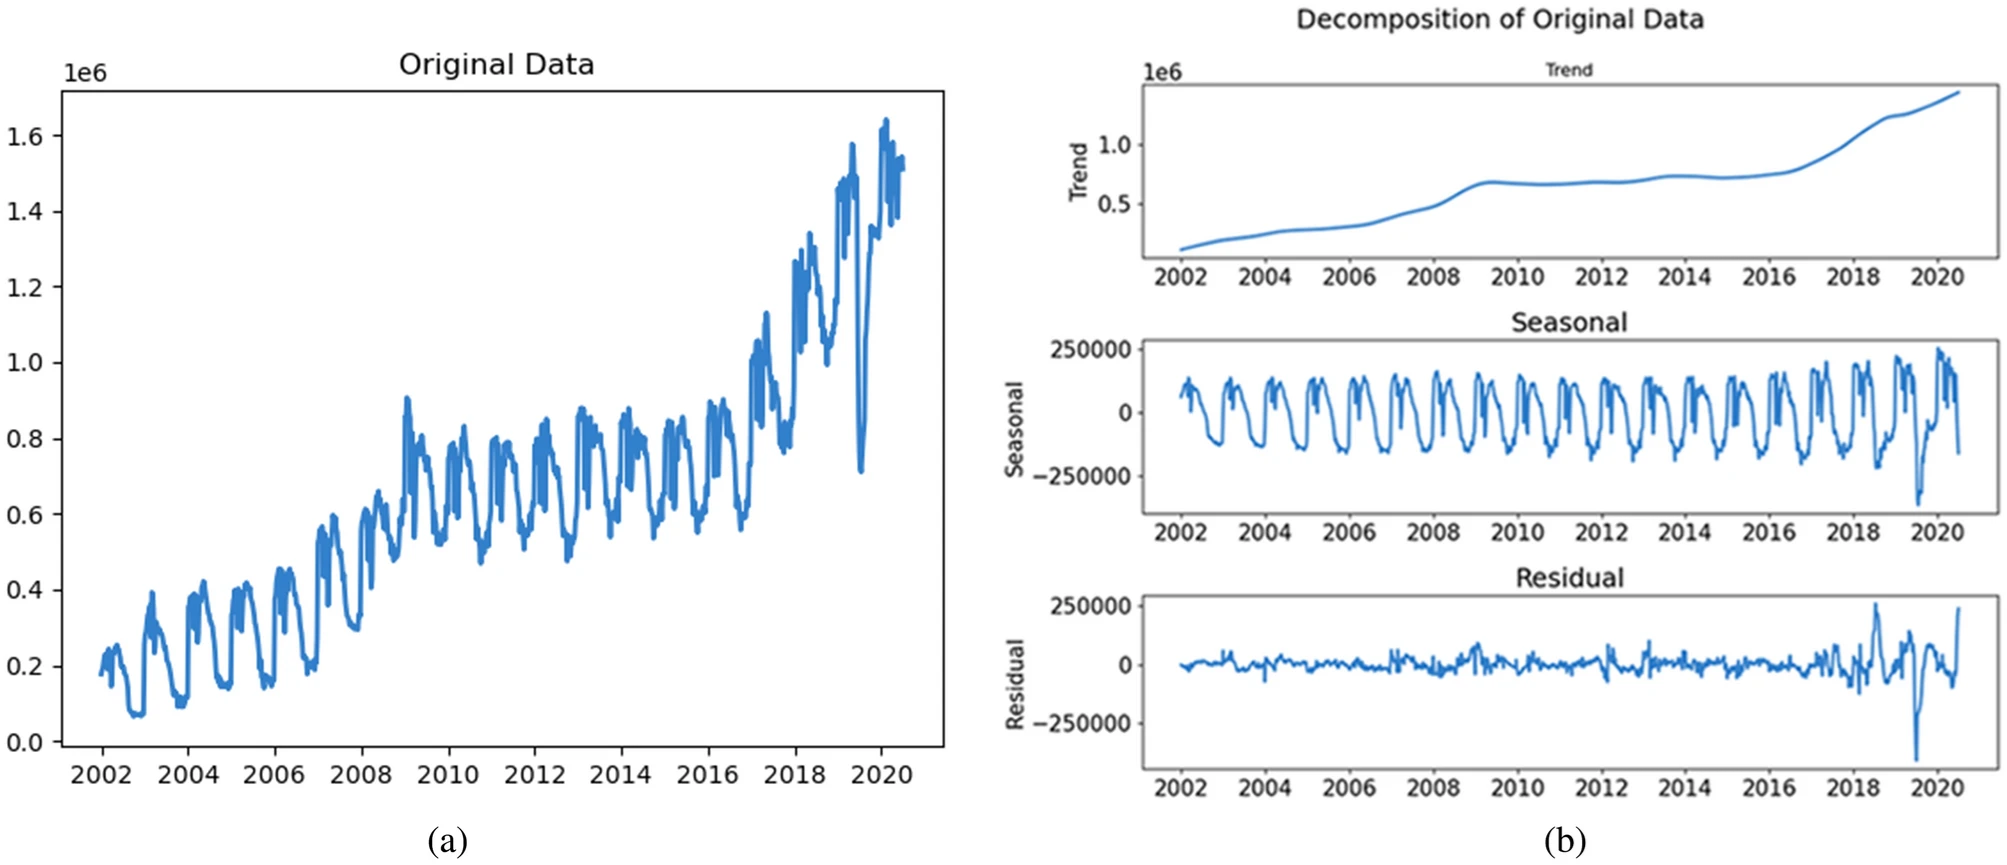
\includegraphics[width=\textwidth]{Pic/Destagionalizzazione.png}
    \end{center}
\end{frame}

\begin{frame}{Definition \cite{brockwell2002introduction}}
\begin{alertblock}{Linear process}
Time series ${X}_{t}$ is a linear process if it has the representation
\begin{equation*}
X_{t}=\sum_{j=-\infty}^{\infty}\psi_{j}Z_{t-j}
\end{equation*}
for all t, where ${Z_{t}}\approx \textrm{WN}(0,\sigma^{2})$ and ${\psi_{j}}$ is a sequence of costants with $\sum_{j=-\infty}^{\infty}\psi_{j} < \infty $. In terms of backward shift operator B $BX_{t}=X_{t-1}$ we have $X_{t}=\phi(B)Z_{t}$ Therefore the previous definition can be rewritten as $X_{t}=\phi(B)Z_{t}$ in which $\phi(B)$ can be thought as a linear filter that when applied to the white noise input series ${Z_{t}}$ produces the output ${X_{t}}$
\end{alertblock}
\end{frame}


\begin{frame}{Definition \cite{brockwell2002introduction}}
\begin{alertblock}{Linear process}
The time series ${X_{t}}$ is an ARMA(1,1) process if its stationary and satisfiy (for every t) 
\begin{equation*}
X_{t}-\phi X_{t-1}=Z_{t}+\theta Z_{t-1}
\end{equation*}
where $Z_{t} \approx \textrm{WN}(0,\phi^{2})$ and $\phi+\theta \neq 0 $
or in terms of filters $\phi$ and $\theta$
\begin{equation*}
\phi(B)X_{t}=\theta(B)Z_{t}
\end{equation*}
\end{alertblock}
\end{frame}

\begin{frame}{Causality \cite{brockwell2002introduction}}
\begin{block}{Remarks}
\begin{itemize}
\item A stationary solution of the ARMA(1,1) equation exists if and only if $\phi \neq \pm 1$
\item If $|\phi| < 1$, then the unique stationary solution is given by $X_{t}=Z_{t}+(\phi+\theta)\sum^{\infty}_{j=1}\phi^{j-1}Z_{t-j}$. In this case we say that $X_{t}$ is causal or a causal function of ${Z_{t}}$ or a causal function of ${Z_{t}}$ since $X_{t}$ can be expressed in terms of the current and past values $Z_{s}$, $s\leq t$
\item If $|\phi| >1$, then the unique stationary solution is given by $X_{t}=-\theta\phi^{-1}Z_{t}-(\phi+\theta)\sum^{\infty}_{j=1}\phi^{-j-1}Z_{t-j}$. The solution is non-causal, since $X_{t}$ is then a functional of $Z_{s}$ $s\geq t$
\end{itemize}
\end{block}
\end{frame}

\begin{frame}{Wold decomposition \cite{brockwell2002introduction}}
\begin{block}{Prediction operator based on the infinite past $X_{t},-\infty < t < n$}
$\tilde{P}_{n}X_{n+h}=\lim_{m\rightarrow - \infty} P_{m,n}X_{n+h}$
\end{block}
\begin{block}{Wold decomposition $X_{t},-\infty < t < n$}
$X_{t}$ is a non-deterministic stationary time series, then
\begin{equation*}
X_{t}=\sum^{\infty}_{j=0}\psi_{j}Z_{t-j}+V_{t}
\end{equation*}
where ${V_{t}}$ is deterministic
\end{block}
\end{frame}

\begin{frame}{Definition \cite{brockwell2002introduction}}
\begin{alertblock}{ARMA (p,q)}
${X_{t}}$ is an ARMA(p,q) process if ${X_{t}}$ is stationary and if for every t, 
\begin{equation*}
X_{t}-\phi_{1} X_{t-1}-...-\phi_{1} X_{t-q}-=Z_{t}+\theta Z_{t}+\theta_{1}Z_{t-1}+...+\theta_{q}Z_{t-q}
\end{equation*}
where ${Z_{t}} \approx WN(0,\sigma^{2})$ and the polynomials $\left(1-\phi_{1}z-...-\phi_{p}z^{p}\right)$ and $\left(1+\phi_{1}z+...+\phi_{p}z^{p}\right)$ have no common factor. 
\end{alertblock}
\end{frame}

\begin{frame}{Definition \cite{brockwell2002introduction}}
\begin{alertblock}{Causality}
An ARMA(p,q) process ${X_{t}}$ is causal, or a causal function of ${Z_{t}}$ if there exist constants  ${\phi_{j}}$ such that $\sum_{j=0}^{\infty}|\phi_{j}|< \infty$ and
\begin{equation*}
X_{t}=\sum^{\infty}_{j=0}\sum\phi_{j}Z_{t-j}\quad\forall\quad t
\end{equation*}
this is equivalent to the condition 
\begin{equation*}
\phi(z)=1-\phi_{1}z-...-\phi_{p}z^{p}\neq \quad|z|<1
\end{equation*}
\end{alertblock}
\end{frame}

\section{Spectral Analysis}


\begin{frame}
\begin{center}
\Huge
Spectral Analysis
\end{center}
\end{frame}



\begin{frame}{Spectral Analysis \cite{brockwell2002introduction}}
\begin{alertblock}{Spectral density}
Given a zero mean stationary time series ${X_{t}}$ with autocovariance function $\gamma()$ satfying $\sum_{h=-\infty}|\gamma(h)|<\infty$, the spectral density of ${X_{t}}$ is the function defined by
\begin{equation*}
f(\lambda)=\dfrac{1}{2\pi}\sum e^{-ih\lambda}\gamma(h)\quad -\infty<\lambda<\infty
\end{equation*}
with the condition that 
\begin{equation*}
f(\lambda)\geq 0 \quad\forall \lambda
\end{equation*}
\begin{equation*}
\gamma(h)=\int^{\pi}_{-\pi}e^{ih\lambda}f(\lambda)d\lambda\forall h
\end{equation*}
\end{alertblock}
\end{frame}

\begin{frame}{Spectral Analysis \cite{brockwell2002introduction}}
\begin{alertblock}{Spectral Representation of The ACVF}
A function $\gamma()$ defined on the integers is the ACVF of a stationary time series if and only if there exists a right-continuous, non-decresing, bounded function F on $[-\pi,\pi]$ with $F(-\pi)=0$ such that:
\begin{equation*}
\gamma(h)=\int_{(-\pi,\pi]}e^{ih\lambda}dF(\lambda)
\end{equation*}
for all integers h. F is a generalized distribution function that is called the spectral distribution function of  $\gamma()$
\end{alertblock}
\end{frame}

\begin{frame}{Spectral Analysis \cite{brockwell2002introduction}}
    \begin{center}
     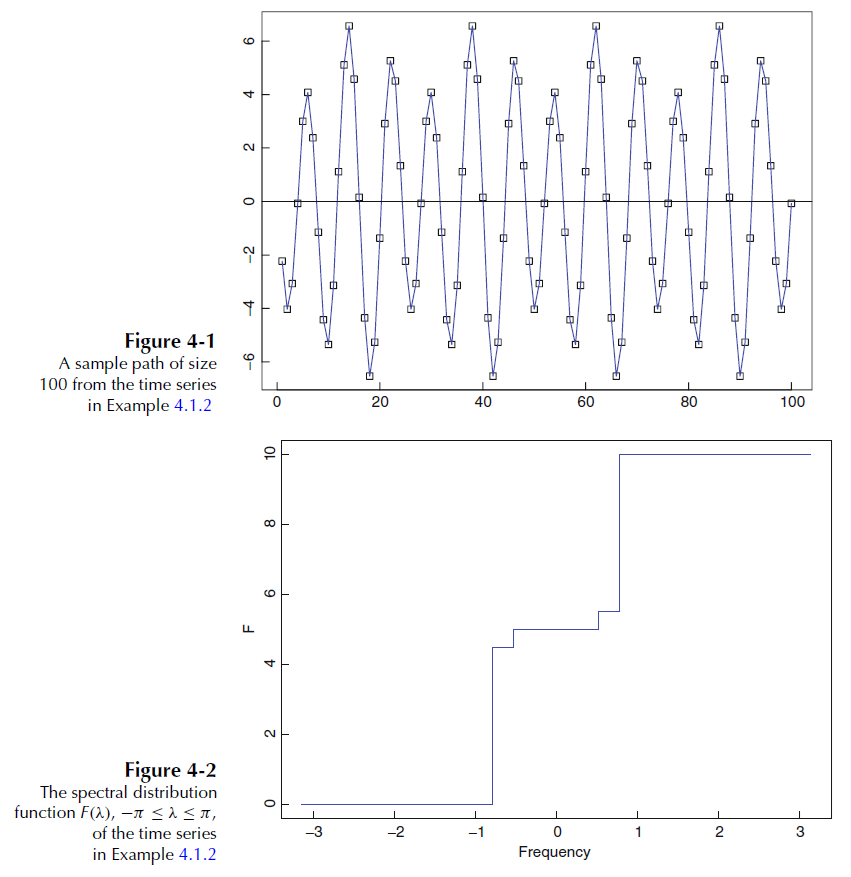
\includegraphics[width=0.6\textwidth]{Pic/spectral_distribution.png}
    \end{center}
\end{frame}


\begin{frame}{Time-Invariant Linear Filters \cite{brockwell2002introduction}}
\begin{alertblock}{Linear process}
The process ${Y_{t}}$ is the output of a linear filter $C=\left\lbrace c_{t,k},t,k=0\pm1,...\right\rbrace$  applied to an input process ${X_{t}}$ if $Y_{t}=\sum^{\infty}_{k=-\infty}c_{t,k}X_{k}\quad t=0,\pm 1,...$
\end{alertblock}
\begin{alertblock}{Time invariant}
The filter is said to be time-invariant if the weights $c_{t,t-k}$ are independent of t e.g. $c_{t,t-k}=\phi_{k}$
\begin{equation*}
Y_{t}=\sum^{\infty}_{k=-\infty}\phi_{t,k}X_{t-k}
\end{equation*}
\begin{equation*}
Y_{t-s}=\sum^{\infty}_{k=-\infty}\phi_{t,k}X_{t-s-k}
\end{equation*}
The TLF $\phi$ is to be causal if $\phi_{j}=0$ for $j<0$
\end{alertblock}
\end{frame}


\begin{frame}{Time-Invariant Linear Filters \cite{brockwell2002introduction}}
\begin{alertblock}{Transfer function}
Let ${X_{t}}$ be a stationary time series with mean zero and spectral density $f_{x}(\lambda)$. Suppose that $\Phi=\left\lbrace \phi_{j},j=0,\pm 1,... \right\rbrace$ is an absolutely summable TLF. Then the time series 
\begin{equation*}
Y_{t}=\sum_{j=-\infty}^{\infty}\phi_{j}X_{t-j}
\end{equation*}
is stationary with mean zero and spectral density 
\begin{equation*}
f_{Y}(\lambda)=|\Psi(e^{-i\lambda})|^{2}f_{X}(\lambda)=\Psi(e^{-i\lambda})\Psi(e^{i\lambda})f_{X}(\lambda)
\end{equation*}
where $\Psi(e^{-i\lambda})=\sum^{\infty}_{j=-\infty}\phi_{j}e^{-ij\lambda}$ where  $\Psi(e^{-i})$ is called the transfer function of the filter, and the squared modulus $|\Psi(e^{-i})|$ is referred to as the power transfer function of the filter. 
\end{alertblock}
\end{frame}

\begin{frame}{Time-Invariant Linear Filters \cite{brockwell2002introduction}}
\begin{exampleblock}{Simple moving average}
\begin{equation*}
Y_{t}=\dfrac{1}{2q+1}\sum_{|j|<q}X_{t-j}
\end{equation*}
where $\psi=(2q+1)^{-1},j=-q,...,q$ and $\psi_{j}$
\end{exampleblock}
    \begin{center}
     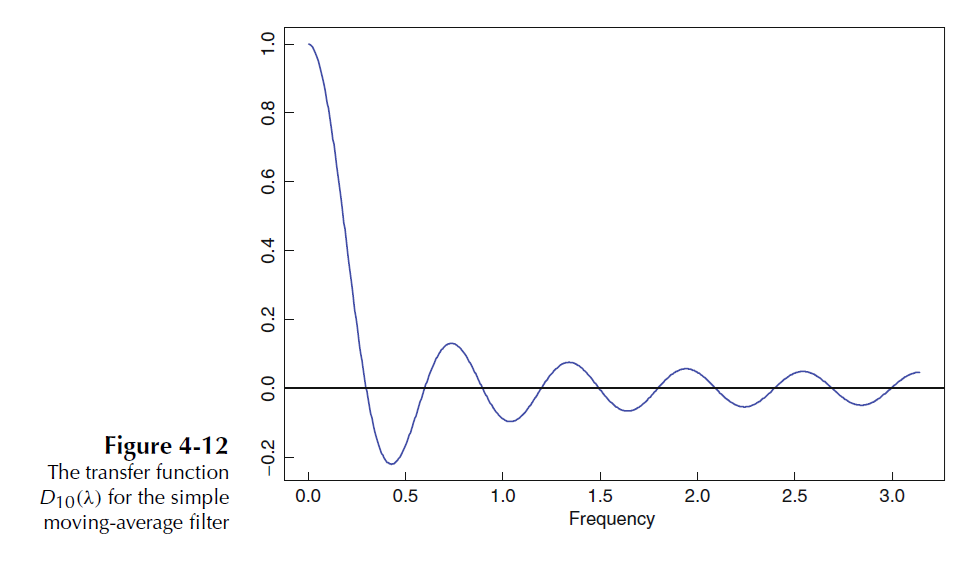
\includegraphics[width=0.6\textwidth]{Pic/D_MA.png}
    \end{center}
\end{frame}

\begin{frame}{Time-Invariant Linear Filters \cite{brockwell2002introduction}}
\begin{exampleblock}{Gibbs phenomenon}
The poor approximation in the neighbourhood of cut-off frequency $(\omega_{c})$ 
\end{exampleblock}
    \begin{center}
     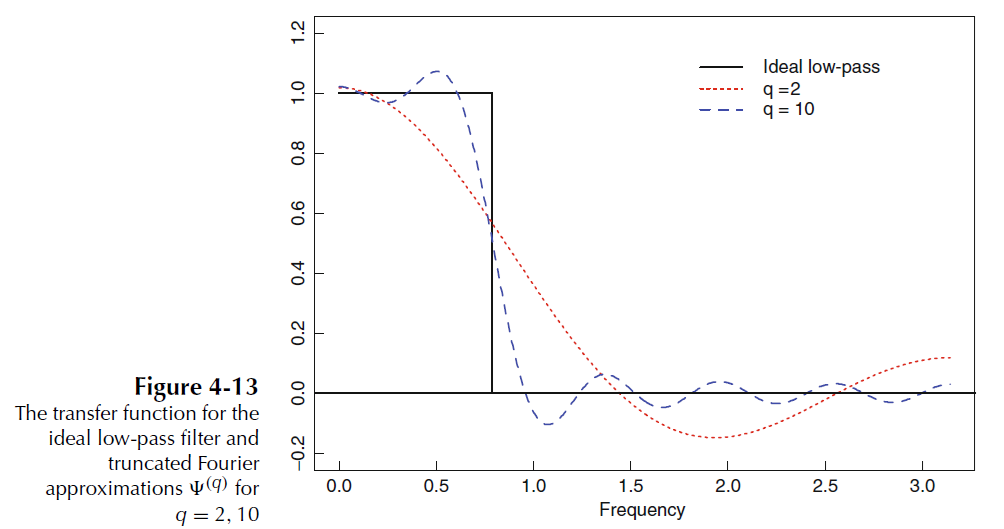
\includegraphics[width=\textwidth]{Pic/gibbs_ph.png}
    \end{center}
\end{frame}


\section{Estimation}
\begin{frame}
\begin{center}
\Huge
Estimation
\end{center}
\end{frame}

\begin{frame}{Esimation \cite{brockwell2002introduction}}
\small
\begin{alertblock}{Gaussian Likehood}
\begin{equation*}
L(\bm{\hat{\phi}},\bm{\hat{\theta}},\bm{\sigma}^{2})=\dfrac{1}{\sqrt{(2\pi\sigma)^{n}r_{0}...r_{n-1})}}\exp(-\dfrac{1}{2\sigma^{2}}\sum \dfrac{(X_{j}-\hat{X_{j}})^{2}}{r_{j-1}})
\end{equation*}
\end{alertblock}
\begin{alertblock}{Maximum Likehood Estimators}
Differentiating $\ln L(\phi,\theta\,\sigma^{2})$ partially with respect to $\sigma^{2}$ and noting that $\hat{X_{j}}$ and $r_{j}$ are independent of $\sigma$
\begin{equation*}
\hat{\sigma}^{2}=n^{-1}S(\bm{\hat{\phi}},\bm{\hat{\theta}})
\end{equation*}
\begin{equation*}
S(\bm{\hat{\phi}},\bm{\hat{\theta}})=\sum^{n}_{j=1}(X_{j}-\hat{X_{j}})^{2}/r_{j-1}
\end{equation*}
where $\bm{\hat{\phi}}$,$\bm{\hat{\theta}}$ are the values of $\bm{\phi}$,$\bm{\theta}$ that minimize:
\begin{equation*}
\mathcal{L}(\phi,\theta)=\ln(n^{-1}S(\phi,\theta))+n^{-1}\sum^{n}_{j=1}\ln r_{j-1}
\end{equation*}

\end{alertblock}

\end{frame}

\begin{frame}{Estimation \cite{brockwell2002introduction}}
\begin{alertblock}{Akaike information criterion}
\begin{equation*}
AICC=-2\ln L(\bm{\hat{\phi}},\bm{\hat{\theta}},S((\phi_{p},\theta_{q})/n)+2(p+q+1)n/(n-p-q-2)
\end{equation*}
\end{alertblock}
\begin{alertblock}{Residual}
\begin{equation*}
\hat{W}_{t}=\left( X_{t} -\hat{X_{t}}\phi,\theta\right)/\left(r_{t-1}( \hat{\phi},\hat{\theta})\right)^{1/2} \quad t=1,...,n 
\end{equation*}
This should have properties similar to the white noise sequence, thus one can define the rescaled residuals
\begin{equation*}
\hat{R}_{t}=\hat{W}_{t}/\hat{\sigma} 
\end{equation*}
\begin{equation*}
\hat{\sigma}=\sqrt{\left(\sum^{n}_{t=1}\hat{W}^{2}_{t}\right)/n}
\end{equation*}
\end{alertblock}
\end{frame}

\begin{frame}{Residuals \cite{brockwell2002introduction}}
    \begin{center}
     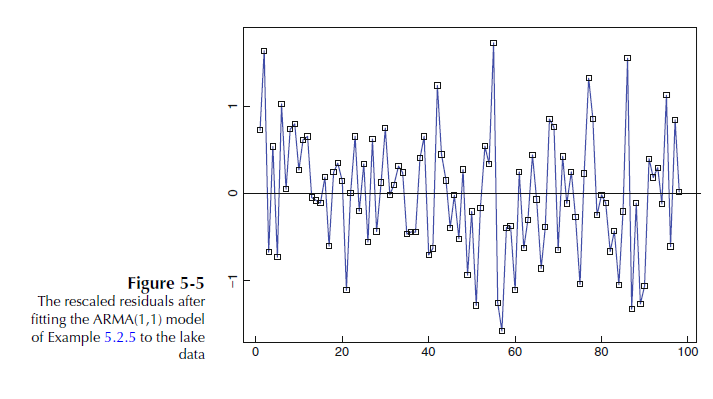
\includegraphics[width=0.8\textwidth]{Pic/Residuals.png}
    \end{center}
\end{frame}

\section{Nonstationary time series}
\begin{frame}
\begin{center}
\Huge
Nonstationary time series
\end{center}
\end{frame}

\begin{frame}{Residuals \cite{brockwell2002introduction,ur}}
    \begin{center}
     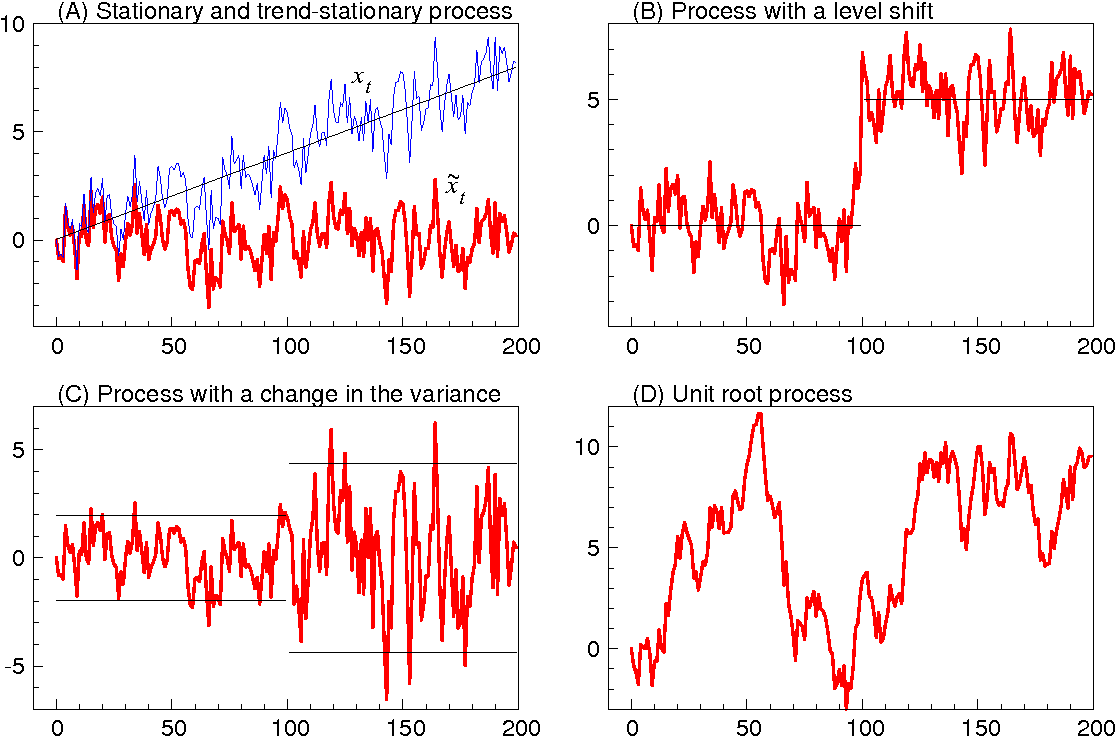
\includegraphics[width=0.8\textwidth]{Pic/unit_root_ts.png}
    \end{center}
\end{frame}

\begin{frame}{Estimation \cite{brockwell2002introduction}}
\begin{alertblock}{Akaike information criterion}
If $d$ is a non-negative integer, then ${X_{t}}$ is an ARIMA(p,d,q) process if 
\begin{equation*}
Y_{t}=(1-B)^{d}X_{t}
\end{equation*}
is causal ARMA(p,q) process $BX_{t}=X_{t-1}$. Note thaat $\nabla X_{t}=X_{t}-X_{t-1}$
\end{alertblock}
\end{frame}

\section{Multivariate time series}
\begin{frame}
\begin{center}
\Huge
Multivariate time series
\end{center}
\end{frame}

\begin{frame}{Multivariate time series \cite{brockwell2002introduction}}
\begin{alertblock}{Akaike information criterion}
$\left\lbrace \textbf{X}_{t} \right\rbrace$ is an ARMA (p,q) process if $\left\lbrace \textbf{X}_{t} \right\rbrace$ is stationary and if for every t, 
\begin{equation*}
\bm{X}_{t}-\phi_{1}\bm{X}_{t-1}-...-\phi_{p}X_{t-p}=Z_{t}+\Theta_{1}Z_{t-1}+...+\Theta_{q}Z_{t-q}
\end{equation*}
where $Z_{t}\approx$ WN(0,$\Sigma$)
\end{alertblock}
\end{frame}

\begin{frame}{Vector Autoregression \cite{hamilton2020time}}
\begin{alertblock}{VAR(1)}
\begin{equation*}
\begin{pmatrix} y_{1,t} \\ y_{2,t} \end{pmatrix} = \begin{pmatrix} c_{1} \\ c_{2} \end{pmatrix} + \begin{pmatrix} a_{1,2}\quad a_{1,2} \\ a_{2,1} \quad a_{2,2} \end{pmatrix} \begin{pmatrix} y_{1,t-1} \\ y_{2,t-1} \end{pmatrix} +
\begin{pmatrix} e_{1,t} \\ e_{2,t} \end{pmatrix}
\end{equation*}
\end{alertblock}

\begin{alertblock}{Granger causality test (hamilton2020time)}
$y_{2}$ cause (in Granger sense) $y_{1}$ if the coefficent $a_{1,2}$ is signficantly not equal to 0
\begin{center}
     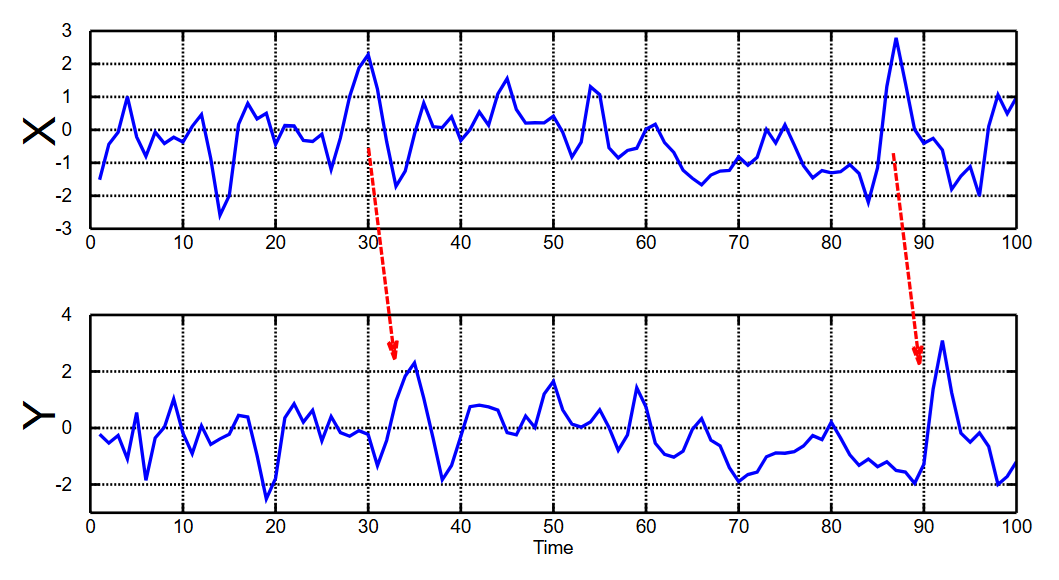
\includegraphics[width=0.5\textwidth]{Pic/granger.png}
    \end{center}
    \end{alertblock}
\end{frame}

\begin{frame}{Vector Autoregression \cite{hamilton2020time}}
\begin{alertblock}{Impulse response function}
$y_{2}$ cause (in Granger sense) $y_{1}$ if the coefficent $a_{1,2}$ is signficantly not equal to 0
\begin{center}
     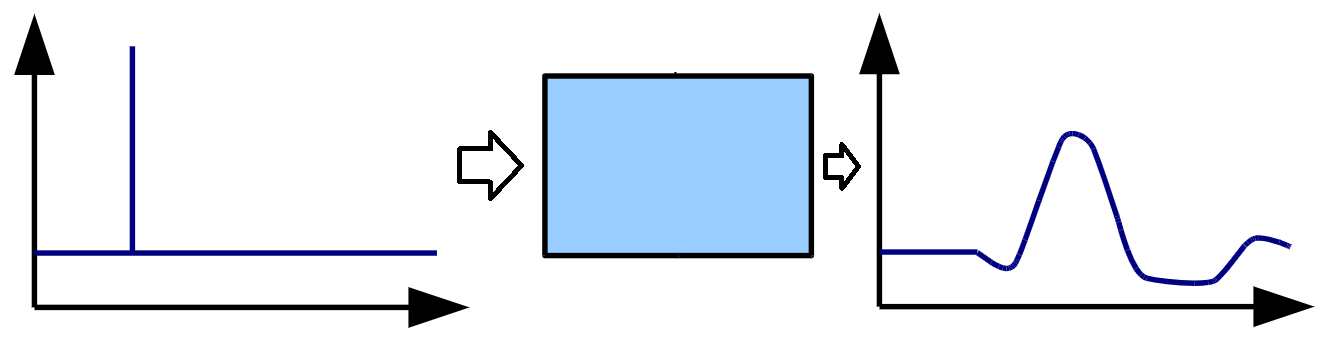
\includegraphics[width=0.8\textwidth]{Pic/irf.png}
    \end{center}
    \end{alertblock}
\end{frame}

\section{State-space models}
\begin{frame}
\begin{center}
\Huge
State-space models
\end{center}
\end{frame}

\begin{frame}{Space State Models  \cite{pml2Book}}
\begin{alertblock}{Definition}
A state-space model (SSM) is a partially observed Markov model in which the hidden state $z_{t}$ evolves over time according to a Markov process and each hidden state generates some observations $y_{t}$ at each step. The main goal is to infer the hidden states given the observations (and also to predict the future observations)
\begin{center}
     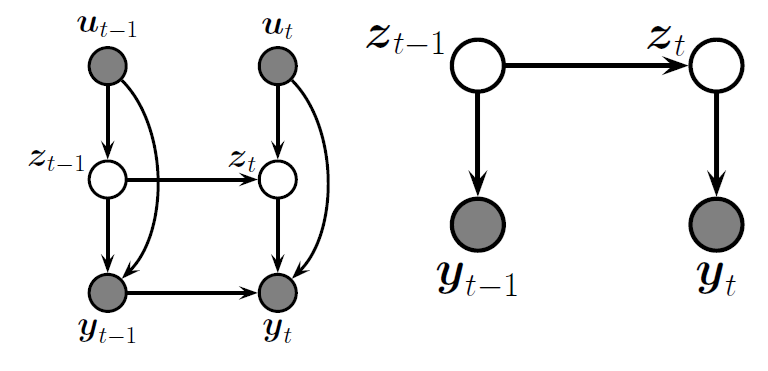
\includegraphics[width=0.6\textwidth]{Pic/SSM.png}
    \end{center}
    \end{alertblock}
\end{frame}

\begin{frame}{Space State Models  \cite{pml2Book}}
\begin{alertblock}{Non linear dynamical system}
A state-space model (SSM) can be represented as a stochastic discrete time nonlinear dynamical system of the form 
\begin{equation*}
\begin{split}
z &= f(\textbf{z}_{t-1},\textbf{u}_{t},\textbf{q}_{t}) \\
y_{t} &= h(\textbf{z}_{t},\textbf{u}_{t},\textbf{y}_{1:t-1},\textbf{r}_{t})
\end{split}
\end{equation*}
where $z_{t} \in 	\mathbb{R}^{N}$ are the hidden states, $\textbf{u}_{t}  \in 	\mathbb{R}^{N}$ are the optional observed inputs, $y\textbf{y}_{t}  \in 	\mathbb{R}^{N}$ are observed output and $\textbf{f}$ is the transition function, $\textbf{q}_{t}$ is the process noise, $\textbf{h}$ is the observation function and $\textbf{r}_{t}$ is the observation noise. The transition model and the observational model are 
\begin{equation*}
\begin{split}
p(\textbf{z}_{t}|\textbf{z}_{t-1},\textbf{u}_{t})& = p(\textbf{z}_{t}|\textbf{f}(\textbf{z}_{t-1},\textbf{u}_{t}))\\
p(\textbf{y}_{t}|\textbf{z}_{t},\textbf{u}_{t},\textbf{y}_{1:t-1})& =p(\textbf{y}_{t}|\textbf{h}(\textbf{z}_{t},\textbf{u}_{t},\textbf{y}_{1:t-1}))
\end{split}
\end{equation*}
\end{alertblock}
\end{frame}

\begin{frame}{Space State Models  \cite{pml2Book}}
\begin{alertblock}{Non linear dynamical system}
Hidden Markov Model (HMM) $\rightarrow$ a SSM in which the hidden states are discrete, thus $z_{t}\in {1,...,K}$
\end{alertblock}
\begin{exampleblock}{Time series segmentation}
\begin{center}
     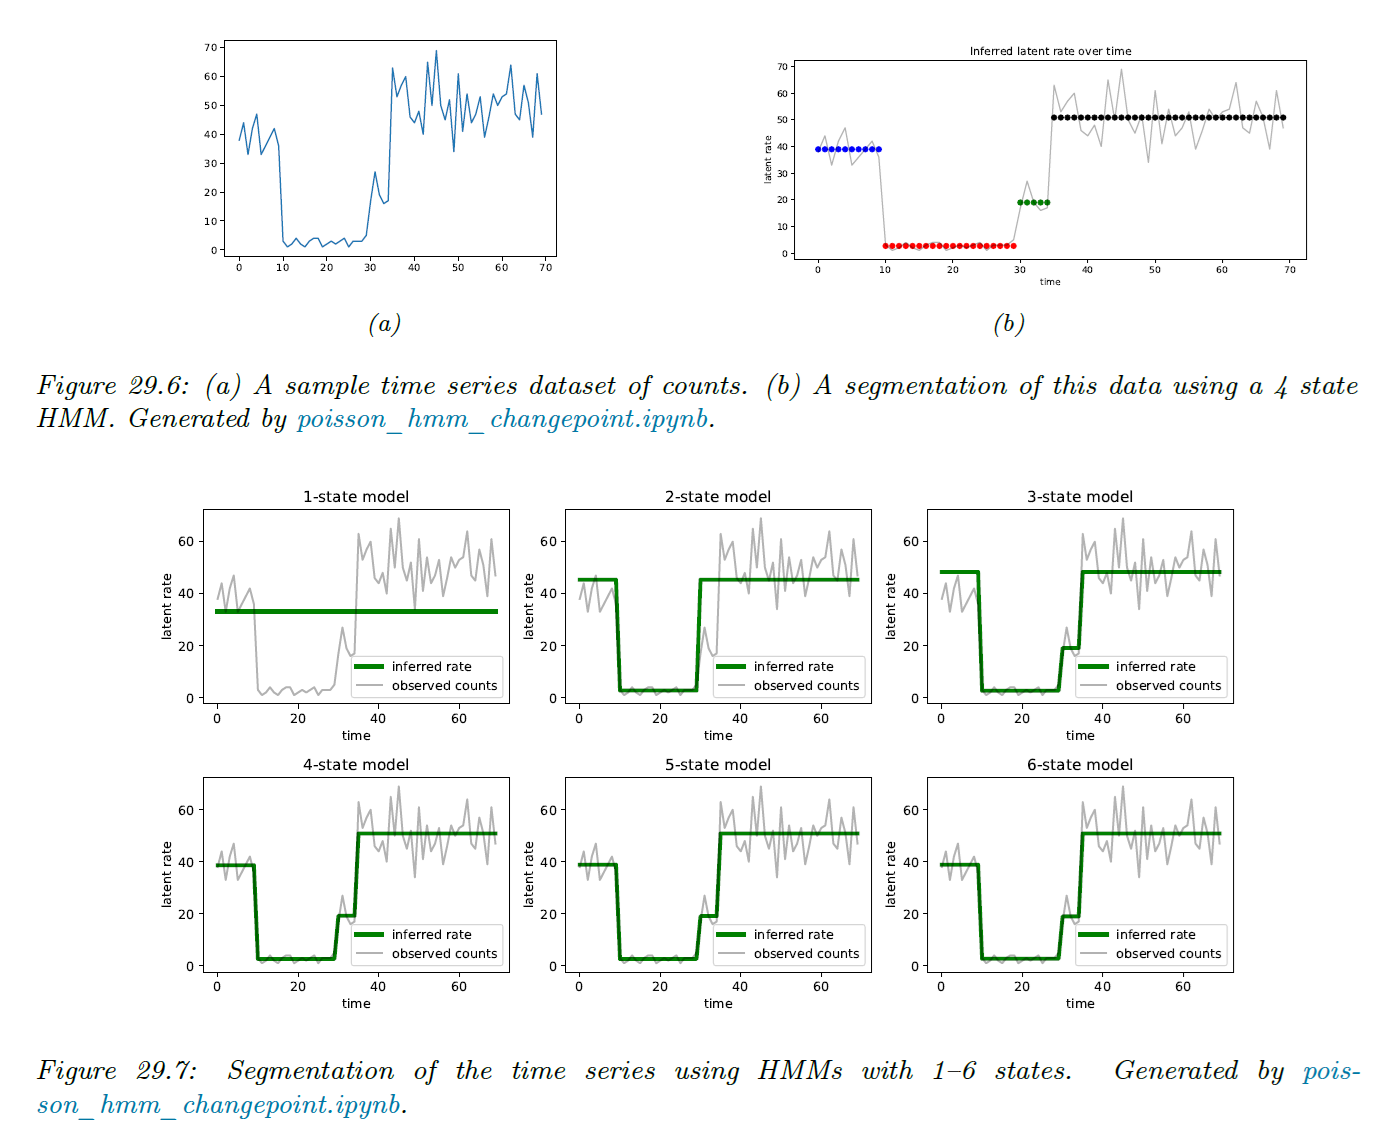
\includegraphics[width=0.5\textwidth]{Pic/time_series_segmentation.png}
    \end{center}
    \end{exampleblock}
\end{frame}

\begin{frame}{Space State Models  \cite{pml2Book}}
\small
\begin{exampleblock}{Time series segmentation}
We want to segment a time series into different regimes, each of which correspond to a different statistical distribution. In particular we would like to segment this data stream in to K different regimes or states, each of which is associated with a Poisson observation model with rate $\lambda_{k}$:
\begin{equation*}
p(y_{t}|z_{t}=k)= Poi\left(y_{t}|\lamda_{k}\right)
\end{equation*}
where a uniform prior over the initial states was considered. The transition matrix will be:
\begin{equation*}
z_{1}\approx \textnormal{Categorical}\left( \left\lbrace \dfrac{1}{4},\dfrac{1}{4},\dfrac{1}{4},\dfrac{1}{4}\right\rbrace \right)
\end{equation*}
\begin{equation*}
z_{1}|z_{t-1}\approx \textnormal{Categorical}\left( \left\lbrace  \begin{pmatrix} p  \quad z_{t}=z_{t-1} \\ \dfrac{1-p}{4-1}  \quad \textnormal{else}  \end{pmatrix}  \right\rbrace \right)
\end{equation*}
\begin{equation*}
p(y_{1:T}|K)\approx \max_{\lambda}\sum p\left( \bm{y}_{1:T},\bm{z}_{1:T}| \bm{\lambda},K \right)
\end{equation*}
\end{exampleblock}
\end{frame}

\begin{frame}{Structural time series models \cite{pml2Book}}
\small
\begin{alertblock}{Structural time series (STS)}
Defined in terms of linear-Gaussian SSMs. Differently from ARMA method, they have much more flexibility: one can create non-linear, non-Gaussian and even hierarchical extension.
Represent the observed scalar time series as a sum of C individual components
\begin{equation*}
f(t)=f_{1}(t)+f(t)+...+f_{C}(t)+\epsilon_{t}
\end{equation*}
Each single component (latent process) $f_{c}(t)$ is modeled by a linear Gaussian state-space model which is also called dynamic linear model. Since these are linear, one can combine in to a single state-space model. 
\begin{equation*}
\begin{split}
p(z_{t}|z_{t-1},\theta)= & \mathcal{N}(z_{t}|Fz_{t-1},Q) \\
p(y_{t}|z_{t},\theta)= & \mathcal{N}(y_{t}|Hz_{t}+\beta^{T}u_{t},\sigma^{2}_{y})
\end{split}
\end{equation*}
where $\bm{F}$ and $\bm{Q}$ are block structure matrices, with one block per component. The vector $\bm{H}$ then adds up all the relevant piecies from each component to generate the overall mean. 
\end{alertblock}
\end{frame}

\begin{frame}{Structural time series models \cite{pml2Book}}
\small
\begin{exampleblock}{Local level model}
The observation $y_{t} \in  \mathbb{R}^{N}$ are generated by a Gaussian with (latent) mean $\mu_{t}$ , which evolves over over time according to a random walk 
\begin{equation*}
\begin{split}
y_{t}=\mu_{t}+\epsilon_{y,t} \quad \epsilon_{y,t}\approx \mathcal{N}(0,\sigma_{y}^{2}) \\
\mu_{t}=\mu_{t-1}+\epsilon_{t-1}_{\mu,t} \quad_{\mu,t} \approx  \mathcal{N}(0,\sigma_{\mu}^{2})
\end{split}
\end{equation*}
One can also assume that $\mu_{1} \in  \mathcal{N}(0,\sigma^{2}_{\mu})$. Thus the latent mean at any future step has distribution $\mu_{t} \in  \mathcal{N}(0,t\sigma^{2}_{\mu}$ so the variance grows with time. Once can also use an autoregressive model in which $\mu_{t}=\rho\mu_{t-1}+\epsilon_{\mu,t}$ where $|\rho<1|$. In this case we have $\mu_{\infty}\approx \mathcal{N}(0,\dfrac{\sigma^{2}_{\mu}}{1-\rho^{2}})$: thus the uncertainty grows to finite asymptote instead of undoubtedly
\end{exampleblock}
\end{frame}

\begin{frame}{Structural time series models \cite{pml2Book}}
\small
\begin{exampleblock}{Space representation of ARMA models}
In this case we have 
\begin{equation}
Z= \begin{pmatrix} Y_{t-p+1} \\ Y_{t-p+2}  \\ ... \\ Y_{t} \end{pmatrix}
\end{equation}
And the observation equation is
\begin{equation}
Y_{t}=[0,0,0,...,1]X_{t} \quad t=\pm 0,\pm 1,...
\end{equation}
And the state equation is 
\begin{equation}
X_{t+1}= \begin{pmatrix} 0 & 1 &  0 &... & 0 \\ 0 & 0 & 1 & ... & 0  \\ ... \\ 0 & 0  & 0 & ... & 1 \\ \phi_{p} & \phi_{p-1} & \phi_{p-2} & ... & \phi_{1} \end{pmatrix} \bm{X}_{t}+ \begin{pmatrix} 0 \\ 0 \\... \\ 0 \\ 1 \end{pmatrix}\textrm{WN}(0,\sigma^{2}) \quad t=0,\pm{1},...
\end{equation}
\end{exampleblock}
\end{frame}


\section{The Kalman Recursions}
\begin{frame}
\begin{center}
\Huge
The Kalman Recursions
\end{center}
\end{frame}


\begin{frame}{The Kalman Recursions \cite{brockwell2002introduction}}
\small
\begin{alertblock}{General idea }
Finding the best (in the sense of minimum square error) linear estimates of the state vector $X_{t}$ in terms of observations $Y_{1}$,$Y_{2}$ and a random vector $Y_{0}$ that is orthogonal to $V_{t}$ and $W_{t}$ for all $t\geq 1$ for these three cases: 
\begin{itemize}
\item $Y_{0},...,Y_{t-1}$ defines the prediction problem
\item $Y_{0},...,Y_{t}$ defines the filtering problem
\item $Y_{0},...,Y_{n}$ ($n > t$) defines the smoothing problem 
\end{itemize}
these problem can be solved useing the Kalman recursion
\end{alertblock}
\begin{alertblock}{Best linear predictor}
For the random vector $X=(X_{1},...,X_{\nu})'$ 
\begin{equation*}
P(X)=(P_{t}(X_{1}),...,P_{t}(X_{\nu}))'
\end{equation*}
where $P_{t}(X)=P(X_{i}|\bm{Y}_{0},\bm{Y}_{1},...,\bm{Y}_{t})$  is the best linear predictor of $X_{i}$ in terms of all components of $\bm{Y}_{0},\bm{Y}_{1},...,\bm{Y}_{t}$
\end{alertblock}
\end{frame}


\begin{frame}{The Kalman Recursions  \cite{brockwell2002introduction}}
\small
\begin{alertblock}{Kalman prediction}
For the state-space model 
\begin{equation*}
\begin{split}
Y_{t} &= G_{t}X_{t}+W_{t} \\
X_{t+1} &= F_{t}X_{t}+V_{t}\\
\end{split}
\end{equation*}
where W and V are two uncorrelated noises. The one-step predictors $\hat{X}_{t}=P_{t-1}(X_{t})$ and their error covariance matrices $\Omega_{t}=E\left[(X_{t}-\hat{X_{t}})(X_{t}-\hat{X_{t}})' \right]$ are uniquely determinated by the initial conditions 
\begin{equation*}
\hat{\bm{X}_{t}}=P(X_{t}|Y_{0}) \quad \Omega_{1}=E\left[\left(\bm{X}_{1}-\hat{\bm{X}}_{1}\right)\left(\bm{X}_{1}-\hat{\bm{X}}_{1}\right)' \right]
\end{equation*}
and the recursion, for $t=1,...,$ 
\begin{equation*}
\begin{split}
\hat{\bm{X}}_{t+1}=&F_{t}\hat{\bm{X}}_{t}+\Theta_{t}\Delta_{t}^{-1}\left( \bm{Y}_{t}-G_{t}\hat{\bm{X}}_{t}  \right) \\
\Omega_{t+1}=&F_{t} \Omega F_{t}'+Q_{t}-\Theta_{t}\Delta_{t}^{-1}\Theta_{t}'
\end{split}
\end{equation*}
where $\Delta_{t}=G_{t}\Omega_{t}G_{t}'+R_{t} \quad \Theta_{t}=F_{t}\Omega_{t}G_{t}'$
\end{alertblock}
\end{frame}




\begin{frame}[noframenumbering,t,allowframebreaks]
\frametitle{Bibliography}
\printbibliography
\end{frame}



\end{document}
